\documentclass[12pt]{article}
\usepackage{ctex}
\usepackage{graphicx}  % 用于插入图片
\usepackage{amsmath}  % 数学公式支持
\usepackage{amssymb}  % 额外数学符号支持
\usepackage{listings}  % 用于插入代码
\usepackage{xcolor}  % 代码高亮
\usepackage{xcolor}    % 用于代码高亮
\usepackage{geometry}  % 用于设置页边距
\usepackage{subcaption}

\lstset{ 
	language=Matlab,                % 设置代码语言
	basicstyle=\ttfamily\footnotesize, % 设置代码字体
	keywordstyle=\color{blue},    % 设置关键词的颜色
	commentstyle=\color{green},   % 设置注释的颜色
	stringstyle=\color{red},      % 设置字符串的颜色
	breaklines=true,              % 自动换行
	frame=single,                 % 给代码加框
	numbers=left,                 % 显示行号
	numberstyle=\tiny\color{gray}, % 设置行号的样式
	stepnumber=1,                 % 每行代码都显示行号
	xleftmargin=0.3in,            % 设置代码块的左边距
	framexleftmargin=0.3in,       % 设置框的左边距
}

\title{作业二~~牛顿插值法实验报告}
\author{姓名: 刘行~~学号: PB22000150}
\date{\today}

\begin{document}
	\maketitle
	\section{实验目的}
		本实验通过牛顿插值法对函数 $f(x) = \frac{1}{1+25x^2}$ 进行插值逼近, 并比较 \textbf{等距插值点} 与 \textbf{切比雪夫插值点} 的误差情况.

	\section{实验原理}
		对于给定的 $N+1$ 个插值点 $(x_0, y_0), (x_1, y_1), \dots, (x_N, y_N)$, 插值多项式可以表示为:
		\begin{equation}
			P_N(x) = f[x_0] + f[x_0, x_1](x - x_0) + \dots + f[x_0, x_1, \dots, x_N](x - x_0)(x - x_1) \dots (x - x_{N-1}),
		\end{equation}
		其中,$f[x_i, x_j, \dots, x_k]$ 是差商,定义为:
		\begin{equation}
			f[x_i] = y_i, \quad f[x_i, x_{i+1}] = \frac{f[x_{i+1}] - f[x_i]}{x_{i+1} - x_i},
		\end{equation}
		\begin{equation}
			f[x_i, x_{i+1}, \dots, x_k] = \frac{f[x_{i+1}, \dots, x_k] - f[x_i, \dots, x_{k-1}]}{x_k - x_i}.
		\end{equation}
	
	牛顿插值多项式具有递归性质,可以通过构造差商表高效地求解.

	\section{代码实现}
		程序主要分为以下几个部分:
		\begin{enumerate}
			\item 定义目标函数 $f(x)$;
			\item 计算牛顿插值多项式;
			\item 选择不同的插值节点;
			\item 计算插值误差并输出.
		\end{enumerate}

		其中牛顿插值多项式由函数 \texttt{function p = newton\_interpolation(x\_nodes, y\_nodes, x\_eval)} 给出, 计算步骤如下:
		\begin{enumerate}
			\item 计算差商表, 存储在上三角矩阵的第一行中.
			\item 递推计算插值多项式的值.
		\end{enumerate} 具体实现如下:

		\begin{lstlisting}[language=Matlab]
function p = newton_interpolation(x_nodes, y_nodes, x_eval)
	N = length(x_nodes);
	divided_diff = y_nodes;
	for j = 2:N
		for i = N:-1:j
			divided_diff(i) = (divided_diff(i) - divided_diff(i-1)) / (x_nodes(i) - x_nodes(i-j+1));
		end
	end
	
	p = divided_diff(N) * ones(size(x_eval));
	for k = N-1:-1:1
		p = divided_diff(k) + (x_eval - x_nodes(k)) .* p;
	end
end
		\end{lstlisting}

		在计算 $N = 20$ 的插值多项式之后将图像输出.

	\section{程序使用说明及实验结果}
		本程序在北太天元软件中编写, 在北太天元界面中直接执行:
		\begin{verbatim}
			>> newton
		\end{verbatim}

		输出结果:
		\begin{verbatim}
N=5
Max Error of grid (1) : 0.4326923077
Max Error of grid (2) : 0.5559113388
N=10
Max Error of grid (1) : 1.9156430502
Max Error of grid (2) : 0.1089290399
N=20
Max Error of grid (1) : 58.2781251077
Max Error of grid (2) : 0.0153250885
N=40
Max Error of grid (1) : 78689.0374850642
Max Error of grid (2) : 0.0002738598
		\end{verbatim}

		对应 $N = 20$ 的函数与插值多项式图像如下图\ref{fig:20}:
		\begin{figure}[htbp]
			\centering
			\begin{subfigure}{0.45\textwidth}
				\centering
				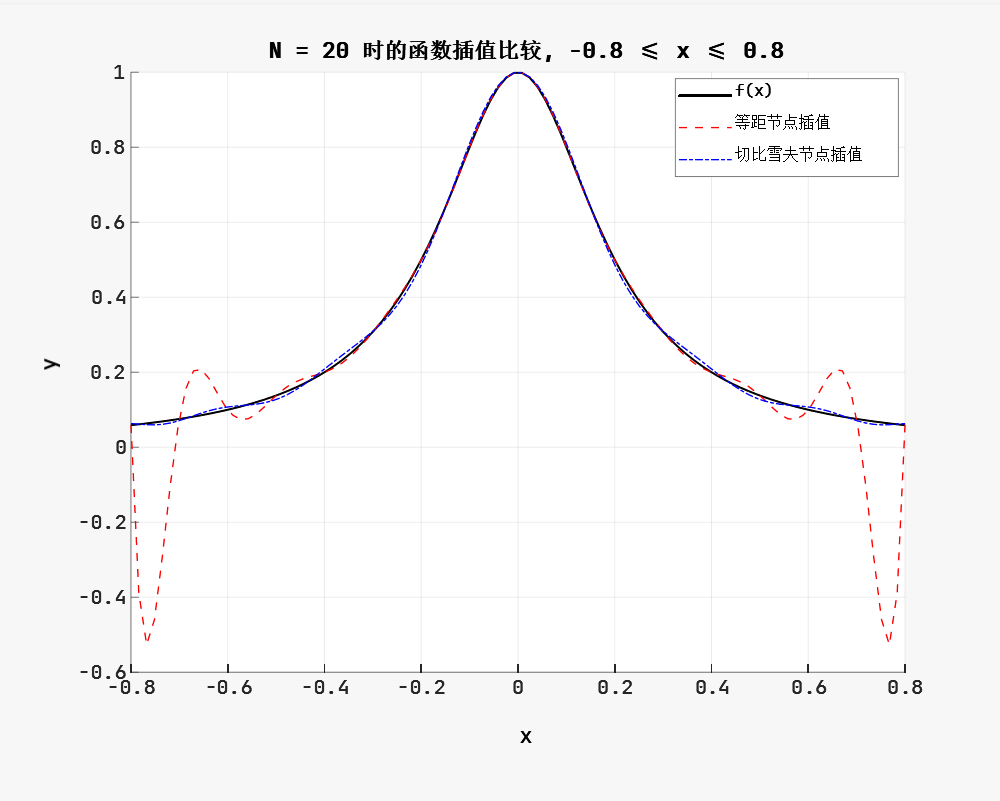
\includegraphics[width=\textwidth]{fig/center.png}
				\caption{center}
				\label{fig:center}
			\end{subfigure}
			\begin{subfigure}{0.45\textwidth}
				\centering
				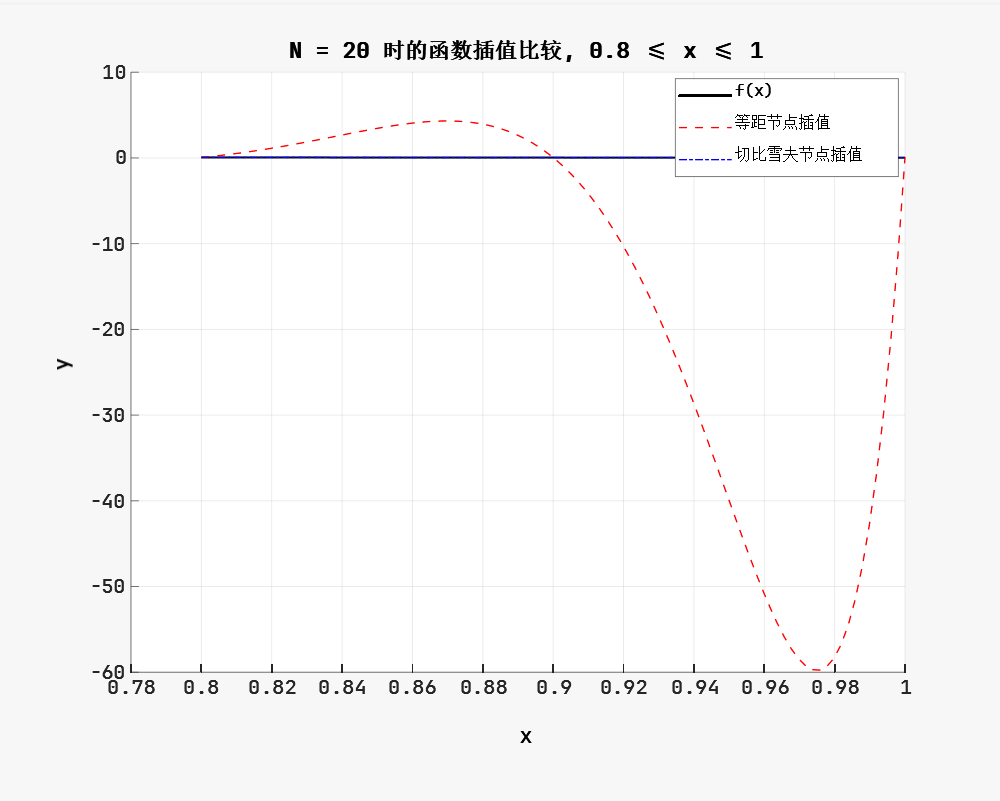
\includegraphics[width=\textwidth]{fig/boundary.png}
				\caption{boundary}
				\label{fig:boundary}
			\end{subfigure}
			\caption{N = 20 图像}
			\label{fig:20}
		\end{figure}

	\section{实验分析}
	从实验结果可以观察到:
	\begin{enumerate}
		\item \textbf{插值误差随 $N$ 增大而减小}, 但等距节点仍存在较大误差, 甚至随着 $N$ 的增大有所增加.
		\item 当 $N = 40$ 时, 切比雪夫插值误差已经非常小, 而等距插值仍然存在较大偏差.
		\item \textbf{切比雪夫节点具有更好的数值稳定性}.
	\end{enumerate}

	\section{结论}
	本实验验证了牛顿插值法在不同插值节点下的误差变化情况。结果表明, \textbf{切比雪夫节点优于等距节点}, 能有效减少误差, 提高插值精度.
\end{document}
